\documentclass[a4paper]{article}

\usepackage[english]{babel}
\usepackage[utf8]{inputenc}
\usepackage{amsmath}
\usepackage{graphicx}
\graphicspath{{/home/jorge/Imágenes/}}
\usepackage[colorinlistoftodos]{todonotes}
\usepackage{amsthm}
\usepackage{amssymb}
\usepackage{nccmath} 
\usepackage{verbatim}
\theoremstyle{definition}
\newtheorem{definition}{Definición}[section]
\newtheorem{example}{Ejemplo}[section]
%% cardinality
\newcommand{\card}[1]{\ensuremath{\lvert #1 \rvert}}

\title{Teoría de Autómatas y Lenguajes Formales\\[.4\baselineskip]Práctica 4: Numeracion de Programas y EXWHILE}


\author{Jorge Ramírez Zotano}

\begin{document}

\maketitle
                                                                                                                                
\section{Menor codigicacion del programa WHILE "diverger" }
Para codificar un progama necesitamos la siguiente funcion que la encontramos en los apuntes en Definition 11.1.7.\\ 
\\ 
Que es : $while2N(Q) = \sigma^2_1\bigl(n, code2N(c)\bigl) $ , donde n es el numero de argunmentos y code2N es el codigo que se va a codificar. \\\\
$code2N(c)=\Gamma\bigl(sent2N(s_1),\dots,sent2N(s_m)\bigl)-1$ , hace una godelizacion a cada linea del codigo.\\
\begin{itemize}
\item $sent2N(c)=\left\{
  \begin{array}{ll}
    5(i-1)                                    & \text{if } c= Xi:=0            \\
    \\ 5\sigma_1^2(i-1,j-1)+1                 & \text{if } c= Xi:=Xj      \\
    \\ 5\sigma_1^2(i-1,j-1)+2                 & \text{if } c= Xi:=Xj+1      \\
    \\ 5\sigma_1^2(i-1,j-1)+3                 & \text{if } c= Xi:=Xj-1   \\
    \\ 5\sigma_1^2\bigl(i-1,code2N(b)\bigl)+4 & \text{if } c= while Xi !=0 do b od \\
  \end{array} \right.$
\end{itemize}
Godelizacion:
\\ 
\begin{center}
$\begin{aligned}
&\Gamma \;:\; \mathbb{N}^* \to \mathbb{N}\\
&\Gamma(\vec{x}) = 
\begin{cases}
 0                         & \text{if } |x| = 0\\
 \sigma^2_1 \left(\card{\vec{x}}-1, \sigma^{\card{\vec{x}}}_1(\vec{x}) \right)+1 & \text{if } \card{\vec{x}} > 0
\end{cases}
\end{aligned}$
\end{center}
\begin{center}
$\begin{aligned}
\text{La funcion dentro de la godelizacion es una cantorizacion de } \mathbb{N}^2\\
\sigma^2_1(x,y) = \frac{(x+y)(x+y+1)}{2}+y\\
\end{aligned}$
\end{center} 
Teniendo ya todos los pasos para encontra la codificacion de un programa solo hay que sustituir\\ 
$while2N(0,"X1:=X1+1;while X1!=0 do X1:=X1 od") $ = 9678230627


\section{Scrip que muestra todos los vectores}
\subsection{Codigo}
function printNvectors(N)\\
for i=0:N-1\\
disp([’(’ num2str(godeldecoding(i)) ’)’])\\
end\\
end\\
\subsection{Ejercucuion}
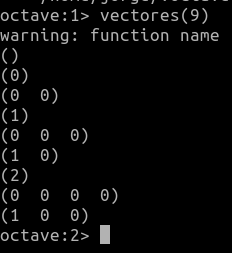
\includegraphics{Nvectores}

\section{Scrip que muestra todos los programas WHILE}
\subsection{Codigo}
function printNwhilePrograms(N)\\
for i=0:N-1\\
disp(N2WHILE(i))\\
end\\
end\\
\subsection{Ejercucuion}
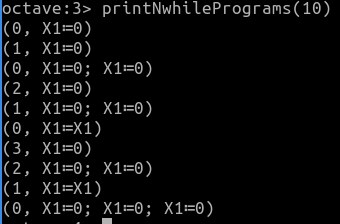
\includegraphics{NProgramas}

\end{document}